% Saturating-activation extension of the fraction-aware two-block theory.
\documentclass[10pt]{article}
\usepackage[margin=0.62in]{geometry}
\usepackage{amsmath,amssymb,booktabs,graphicx}
\usepackage[hidelinks]{hyperref}
\setlength{\parindent}{0pt}
\setlength{\parskip}{3pt}
\setlength{\abovedisplayskip}{4pt}
\setlength{\belowdisplayskip}{4pt}
\setlength{\textfloatsep}{7pt}
\setlength{\floatsep}{6pt}
\renewcommand{\arraystretch}{1.08}

\title{\vspace{-1.3cm}\textbf{Two-Block Circuit Competition with ReLU(tanh) Neurons}}
\author{}
\date{\vspace{-1.15cm}}

\begin{document}
\maketitle
\vspace{-0.75cm}

\textbf{Summary.}
We repeat the fraction-aware two-block derivation for
$\phi(z)=\operatorname{ReLU}(\tanh z)=[\tanh z]_+$.  The steps and notation match the
pure-ReLU theory, but saturation removes positive homogeneity.  Consequently, neuron counts
no longer cancel from the weight-decay cost, the lower-mode leakage ratios depend on the
neuron amplitude, and direct and compositional block-2 circuits can coexist when their
fractions are constrained.  The familiar accessibility boundary $P/S=1/\sqrt8$ survives only
as the weak-activation onset criterion.  We show both the phase diagram conditional on fixed
fractions and the result of minimizing the same free energy over the fractions themselves.

\section*{1. Model, circuit populations, and assumptions}
We keep exactly the objective and residual architecture of the ReLU report:
\begin{align}
h_1&=h_0+\phi(V_1h_0),&h_2&=h_1+\phi(V_2h_1),\nonumber\\[-5pt]
\mathcal J&=\frac{\gamma_2}{2}\!\sum_{a\in\{12,34\}}(1-\widehat A_a)^2
+\frac{\gamma_4}{2}(1-\widehat A_4)^2
+\frac12\!\left(\lambda_E\|E\|^2+\lambda_1\|V_1\|^2+\lambda_2\|V_2\|^2\right.\nonumber\\[-2pt]
&\hspace{4.8cm}\left.+\lambda_p\|W_{d2}\|^2+\lambda_4\|w_4\|^2\right),
\label{eq:objective}
\end{align}
where $\widehat A_a=\mathbb E[f_a\chi_a]$.  Since $\chi_a^2=1$, the aligned pure-mode
loss is $(1-\widehat A_a)^2$ for either target sign.  The available populations are
\begin{align}
&m_{12}=N_1\rho^{(1)}_{2\times1},\qquad
m_{14}=N_1\rho^{(1)}_{4\times1},\nonumber\\[-2pt]
&m_{22}=N_2\rho^{(2)}_{2\times1},\qquad
m_D=N_2\rho^{(2)}_{4\times1},\qquad
m_C=N_2\rho^{(2)}_{2\times2},
\label{eq:counts}
\end{align}
with the unlisted fraction idle or untracked.  The $2\times1$ populations are split equally
between the two canonical parent pairs.

For a balanced neuron with $p$ binary parent modes $y_i\in\{\pm1\}$, write
$z=\xi\sum_{i=1}^{p}y_i$.  Every Walsh coefficient is exactly
\begin{equation}
c_A(\xi)=2^{-p}\sum_{y\in\{\pm1\}^p}
\left[\tanh\!\left(\xi\sum_i y_i\right)\right]_+
\prod_{i\in A}y_i.
\label{eq:walsh}
\end{equation}
For a two-input gate, the constant, two parents, and product all have magnitude
\begin{equation}
a(\xi)=\frac{\tanh(2\xi)}4.
\label{eq:a}
\end{equation}
For a four-input gate, put $t_j=\tanh(j\xi)$.  The coefficients at degrees
$0,1,2,3,4$ are, respectively,
\begin{equation}
b_0=\frac{t_4+4t_2}{16},\quad
b_1=\frac{t_4+2t_2}{16},\quad
b_2=\frac{t_4}{16},\quad
b_3=\frac{t_4-2t_2}{16},\quad
-b_4=\frac{t_4-4t_2}{16},
\label{eq:b}
\end{equation}
where $b_4=(4t_2-t_4)/16>0$ denotes the target magnitude.  Equations
\eqref{eq:a}--\eqref{eq:b} were checked by direct enumeration of the $2^p$ inputs.  As
$\xi\to0$, $(a,b_1,b_2,b_4)\sim(\xi/2,\xi/2,\xi/4,\xi/4)$, reproducing the ReLU
ratios.  As $\xi\to\infty$, they approach $(1/4,3/16,1/16,3/16)$: the ratios are no
longer fixed.

We retain the ReLU report's orthogonal-mode, orthogonal-population, sign-balance,
aligned-readout, sufficient-width, and global-minimum assumptions.  The additional closure
is (A8): neurons in one listed population are exchangeable and have a common $\xi$.  This is
exact for a constrained homogeneous population and gives the simplest finite-fraction
theory.  If amplitudes within a four-input population are unrestricted, their distribution is
an additional order parameter; the final paragraph states the exact replacement.

\section*{2. What changes in the fraction step}
Let every parent coefficient vector have norm $R$.  A balanced $p$-input neuron with
preactivation amplitude $\xi$ has incoming norm $\sqrt p\,\xi/R$.  Thus $m$ identical
neurons producing coefficient magnitude $c(\xi)$ obey
\begin{equation}
Q^2=m c(\xi)^2,\qquad
\frac{\lambda}{2}\sum_{j=1}^{m}\|v_j\|^2
=\frac{\lambda mp}{2R^2}\xi^2.
\label{eq:population}
\end{equation}
For a two-input population, $a^{-1}(u)=\tfrac12\operatorname{arctanh}(4u)$, so eliminating
$\xi$ gives
\begin{equation}
\boxed{\mathcal C_{2,m}(Q;R)=
\frac{\lambda m}{4R^2}\operatorname{arctanh}^2\!\left(\frac{4Q}{\sqrt m}\right)},
\qquad Q<\frac{\sqrt m}{4}.
\label{eq:c2}
\end{equation}
For a four-input target population,
\begin{equation}
\boxed{\mathcal C_{4,m}(Q;R)=
\frac{2\lambda m}{R^2}\left[b_4^{-1}\!\left(\frac{Q}{\sqrt m}\right)\right]^2},
\qquad Q<\frac{3\sqrt m}{16},
\label{eq:c4}
\end{equation}
where the monotone inverse is evaluated numerically.  Unlike the quadratic ReLU costs,
Eqs.~\eqref{eq:c2}--\eqref{eq:c4} depend on $m=N\rho$ and diverge at the saturation
capacity.  Expanding $\operatorname{arctanh}$ and $b_4^{-1}$ at small $Q/\sqrt m$ recovers
the fraction-independent ReLU costs.  This identifies the physical distinction: changing a
positive fraction does nothing in a homogeneous activation, but changes both marginal cost
and capacity once the activation saturates.

The ReLU winner-take-all target-strength result also changes.  With a fixed total block-2
target norm, putting everything into the cheaper linear route was optimal.  Here each route's
marginal cost rises toward its capacity, so the initially cheaper route can be joined by the
other route.  The relevant observable remains the target-strength share
\begin{equation}
\alpha_C\equiv\frac{Q_C^2}{Q_D^2+Q_C^2},
\label{eq:alpha}
\end{equation}
but $\alpha_C$ can now lie strictly between zero and one at $T=0$.

\section*{3. Coupled mode geometry and reduced free energy}
Following the ReLU derivation, retain $s$ for the residual input-singleton norm.  Replace its
four learned strengths by five population amplitudes
$\xi_{12},\xi_{14},\xi_{22},\xi_D,\xi_C$.  The corresponding target strengths are
\begin{align}
q&=\sqrt{m_{12}/2}\,a(\xi_{12}),&
r&=\sqrt{m_{14}}\,b_4(\xi_{14}),&
p&=\sqrt{m_{22}/2}\,a(\xi_{22}),\nonumber\\[-2pt]
Q_D&=\sqrt{m_D}\,b_4(\xi_D),&
Q_C&=\sqrt{m_C}\,a(\xi_C).
\label{eq:strengths}
\end{align}
The new feature is amplitude-dependent leakage.  Define
\begin{equation}
L_1=\sqrt{m_{14}}\,b_1(\xi_{14}),\qquad
L_2=\sqrt{m_{14}}\,b_2(\xi_{14}),\qquad
L_D=\sqrt{m_D}\,b_2(\xi_D).
\label{eq:leakage}
\end{equation}
The input singleton norm $S$, canonical-parent norm $P$, final parent norm $Z$, and final
target norm $H$ are then
\begin{equation}
\boxed{S^2=s^2+q^2+L_1^2,\quad P^2=q^2+L_2^2,\quad
Z^2=P^2+p^2+L_D^2+Q_C^2,\quad H^2=r^2+Q_D^2+Q_C^2.}
\label{eq:geometry}
\end{equation}
This is the direct analogue of $(S^2,P^2)=(s^2+q^2+4r^2,q^2+r^2)$, now with the
correct nonlinear ratios.  Four cross-pair $d2$ modes and the $d3$ modes from the block-1
four-input population are also present, with norms $L_2$ and
$\sqrt{m_{14}}|b_3(\xi_{14})|$; under the orthogonal-readout closure they enter neither
supervised readout and have no downstream block.

Minimizing the two readouts at fixed hidden representation is unchanged:
\begin{equation}
B^*=\frac{\gamma_2Z^2}{\gamma_2Z^2+\lambda_p},\qquad
A^*=\frac{\gamma_4H^2}{\gamma_4H^2+\lambda_4}.
\label{eq:readouts}
\end{equation}
Substitution into Eq.~\eqref{eq:objective} gives the single joint free energy
\begin{align}
F=\min_{s,\,\xi_{12},\xi_{14},\xi_{22},\xi_D,\xi_C\geq0}\Bigg\{&
2\lambda_Es^2
+\frac{\lambda_1}{s^2}\left(m_{12}\xi_{12}^2+2m_{14}\xi_{14}^2\right)\nonumber\\[-2pt]
&+\lambda_2\left(\frac{m_{22}\xi_{22}^2+2m_D\xi_D^2}{S^2}
+\frac{m_C\xi_C^2}{P^2}\right)
+\frac{\gamma_2\lambda_p}{\gamma_2Z^2+\lambda_p}
+\frac{\gamma_4\lambda_4}{2(\gamma_4H^2+\lambda_4)}\Bigg\}.
\label{eq:free}
\end{align}
All quantities in Eq.~\eqref{eq:free} are defined by
Eqs.~\eqref{eq:a}, \eqref{eq:b}, and \eqref{eq:strengths}--\eqref{eq:geometry}.  This is
one simultaneous minimization; its written order is only algebraic convenience.  It includes
both block-2 target routes at once, so it does not presume the answer to the circuit
competition.

As a check, use the small-$\xi$ limits in Eq.~\eqref{eq:free}.  The first-block costs become
$8\lambda_1q^2/s^2+32\lambda_1r^2/s^2$, the block-2 parent cost becomes
$8\lambda_2p^2/S^2$, and the two target costs become
\begin{equation}
32\lambda_2\frac{Q_D^2}{S^2}+4\lambda_2\frac{Q_C^2}{P^2}
=\frac12\left(\kappa_DQ_D^2+\kappa_CQ_C^2\right),\qquad
\kappa_D=\frac{64\lambda_2}{S^2},\quad \kappa_C=\frac{8\lambda_2}{P^2}.
\label{eq:relu-limit}
\end{equation}
Thus the derivation reduces term-by-term to the previous ReLU theory.

\section*{4. Phase diagram and control implications}
At infinitesimal target amplitude, composition first becomes cheaper when
\begin{equation}
\boxed{\kappa_C<\kappa_D\quad\Longleftrightarrow\quad P/S>1/\sqrt8.}
\label{eq:onset}
\end{equation}
At finite amplitude Eq.~\eqref{eq:onset} is not the phase boundary: $b_1:b_2:b_4$ changes
with $\xi$, the two route costs have different curvature and capacities, and their parent
byproducts change the rest of the objective.  The phase is instead read from the minimizer of
Eq.~\eqref{eq:free}: $C$-dominant if $\alpha_C>0.9$, $D$-dominant if
$\alpha_C<0.1$, and mixed otherwise, with separate block-1-only, parent-only, and suppressed
regions.

\begin{figure}[h!]
\centering
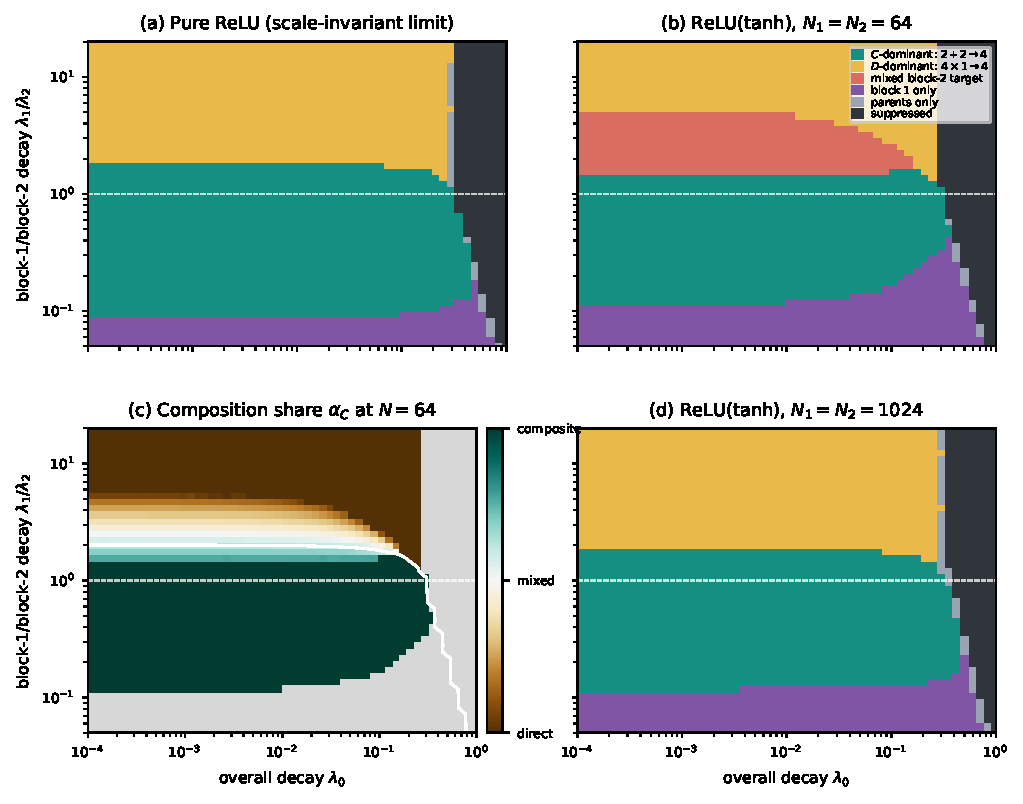
\includegraphics[width=0.73\textwidth]{fig_two_block_relu_tanh_neuron_fraction_phase.pdf}
\vspace{-8pt}
\caption{\textbf{Fixed-fraction homogeneous-population phase diagrams.}
$\gamma_2=\gamma_4=2$ and
$\lambda_E=\lambda_p=\lambda_4=\lambda_2=\lambda_0$; the vertical coordinate is
$\lambda_1/\lambda_2$.  Panels (b)--(d) use
$(\rho^{(1)}_{2\times1},\rho^{(1)}_{4\times1})=(1/2,3/8)$ and
$(\rho^{(2)}_{2\times1},\rho^{(2)}_{4\times1},\rho^{(2)}_{2\times2})=(1/16,1/8,1/4)$.
(a) Pure-ReLU reference. (b) At finite width, saturation produces a genuine mixed strip and
moves the direct/compositional crossover. (c) Composition share; gray means no active
block-2 target.  The white line is $P/S=1/\sqrt8$ and is only the weak-signal diagnostic.
(d) Multiplying every population size by 16 moves each neuron into its linear regime, shrinks
the mixed strip, and approaches panel (a).  Each panel is a multistart numerical minimization
of the displayed reduced free energy.}
\label{fig:phase}
\end{figure}

\textbf{Minimizing over the fractions.}
Within A8, the fractions are ordinary additional order parameters.  Define the two allocation
simplices
\begin{equation}
\Delta_1=\{(\rho_{12},\rho_{14})\!:\rho_{12},\rho_{14}\geq0,
\ \rho_{12}+\rho_{14}\leq1\},\qquad
\Delta_2=\{(\rho_{22},\rho_D,\rho_C)\!:\rho_c\geq0,
\ \rho_{22}+\rho_D+\rho_C\leq1\}.
\label{eq:simplices}
\end{equation}
The unused mass is idle.  The fully optimized homogeneous theory is simply
\begin{equation}
\boxed{F_{\rm opt}=\min_{\rho^{(1)}\in\Delta_1,\,\rho^{(2)}\in\Delta_2}
F\big(\rho^{(1)},\rho^{(2)}\big),}
\label{eq:fopt}
\end{equation}
where $F$ is the simultaneous amplitude minimization in Eq.~\eqref{eq:free} and
$m_{\ell c}=N_\ell\rho^{(\ell)}_c$.  Thus the plotted calculation has only eleven scalar
order parameters: $s$, five amplitudes, and five independent fractions.  We solve them jointly,
not by first optimizing $F$ at arbitrarily fixed features.  A fraction assigned to a population
with $\xi_c=0$ is physically unidentifiable; in Fig.~\ref{fig:optimized-fractions} such mass is
absorbed into the idle category.  For numerical display, a population is called active only if
its propagated modes contribute at least $0.5\%$ of the relevant retained mode norm.

\begin{figure}[h!]
\centering
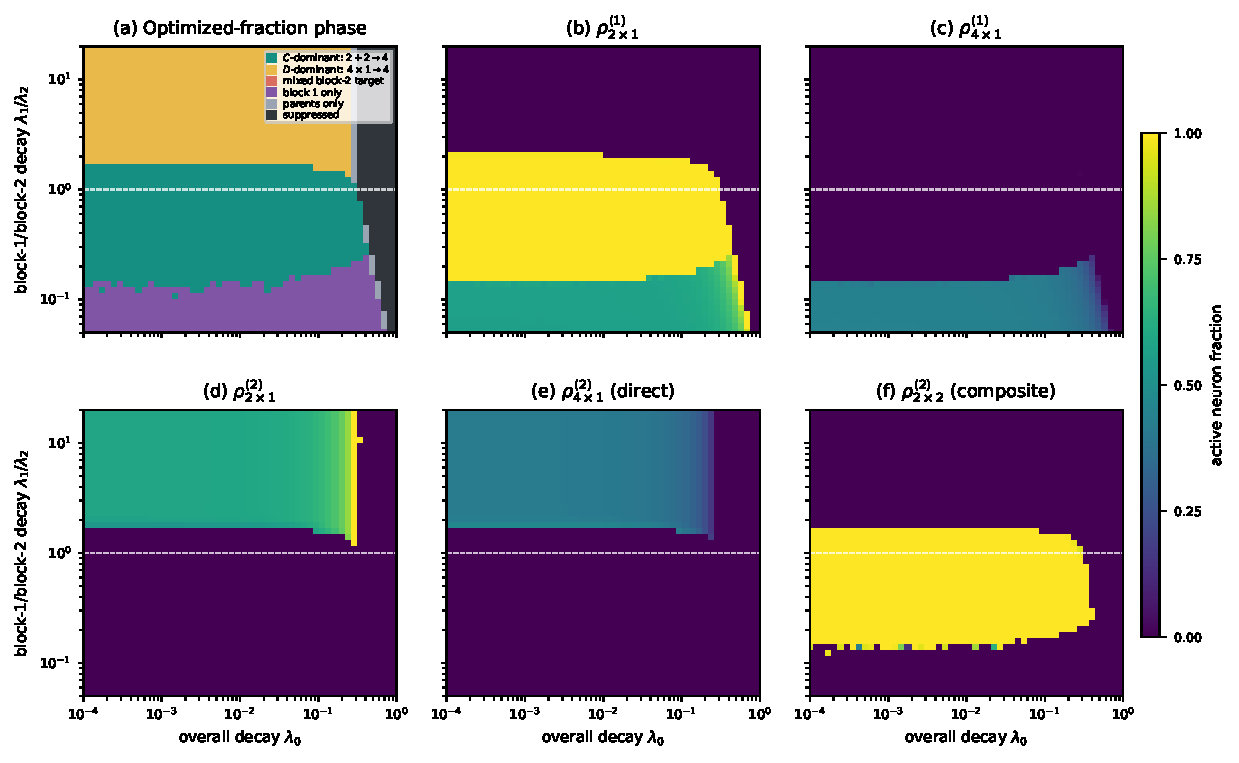
\includegraphics[width=0.91\textwidth]{fig_two_block_relu_tanh_optimized_fraction_phase.pdf}
\vspace{-7pt}
\caption{\textbf{Phase and active fractions after minimizing Eq.~\eqref{eq:fopt}.}
$N_1=N_2=64$ and all loss weights and decay conventions match Fig.~\ref{fig:phase}.
(a) The optimized phase.  (b)--(c) Active first-block fractions.  (d)--(f) Active second-block
fractions.  Unshown mass is idle.  In this slice the optimizer finds no stable mixed block-2
target phase: allowing the allocation to move relieves the fixed-capacity saturation that made
the mixed strip in Fig.~\ref{fig:phase}(b).  The diagrams are multistart numerical global-search
approximations to the displayed eleven-dimensional free energy.}
\label{fig:optimized-fractions}
\end{figure}

Away from phase boundaries the allocation has a simple interpretation.  In the compositional
phase the numerical median is
$(\rho^{(1)}_{2\times1},\rho^{(1)}_{4\times1})\simeq(1,0)$ and
$(\rho^{(2)}_{2\times1},\rho^{(2)}_{4\times1},\rho^{(2)}_{2\times2})\simeq(0,0,1)$.
In the high-$\lambda_1/\lambda_2$ direct phase block 1 is inactive and block 2 splits as
$(0.59,0.41,0)$ between parent and direct-target neurons.  In the block-1-only phase the first
block splits as $(0.565,0.435)$ and block 2 is idle.  These are energy-minimizing active
fractions within A8, rather than fitted inputs or predictions of training dynamics.

\textbf{How decay controls the circuit.}
Increasing $\lambda_1/\lambda_2$ suppresses the block-1 parent representation and favors the
direct $4\times1$ route; making block 1 sufficiently cheap instead lets it solve $d4$ itself.
Between these regimes, preserving $P/S$ favors $2+2\to4$.  Unlike pure ReLU, the result also
depends on the available counts: increasing $m_C$ raises the compositional capacity and
lowers its finite-amplitude marginal cost, while increasing $m_D$ does the same for the direct
route.  Therefore no fraction-independent finite-amplitude boundary exists when fractions are
externally constrained.  If neurons can freely change type, Eq.~\eqref{eq:fopt} predicts the
allocation and, in the displayed slice, removes the mixed strip.  In the large-width or
weak-activation limit, Eq.~\eqref{eq:onset} and the sharp pure-ReLU diagram are recovered.

Finally, A8 is a closure rather than a consequence of the activation.  Without it, replace
each common amplitude by a probability measure $\nu_c(d\xi)$ and replace, for example,
$m_cb_k(\xi_c)^2$ by $m_c\int b_k(\xi)^2\nu_c(d\xi)$ and
$m_c\xi_c^2$ by $m_c\int\xi^2\nu_c(d\xi)$.  Minimizing Eq.~\eqref{eq:free} over these
measures is the exact zero-temperature population theory.  Equal sharing is optimal for the
two-input cost in Eq.~\eqref{eq:c2}; a four-input population can instead split into inactive
and finite-amplitude subpopulations because $[b_4^{-1}(\sqrt{x})]^2$ is not globally convex.
This refinement can change the numerical fractions and phase boundaries.  The robust
conclusions are that saturation makes active fractions physical, constrained capacities can
permit mixed block-2 solutions, and the ReLU boundary is restored as $N\rho\to\infty$ at fixed
aggregate mode norm.

\end{document}
